\documentclass[letterpaper,twocolumn,10pt]{article}
\usepackage{usenix-2020-09}

%\IEEEoverridecommandlockouts
% The preceding line is only needed to identify funding in the first footnote. If that is unneeded, please comment it out.
% \usepackage{cite}
\usepackage{algorithmic}
\usepackage{graphicx}
\usepackage{textcomp}
\usepackage{xcolor}
\def\BibTeX{{\rm B\kern-.05em{\sc i\kern-.025em b}\kern-.08em
    T\kern-.1667em\lower.7ex\hbox{E}\kern-.125emX}}

%\usepackage{newpxtext,newpxmath}
\usepackage{newpxmath}
\usepackage{multirow}
\usepackage{url}
\usepackage{amsmath, amsfonts}
\newcommand{\stitle}[1]{\vspace{1ex}\noindent\textbf{#1}}
\newcommand{\ignore}[1]{}

\newcounter{JohnNOC}
\stepcounter{JohnNOC}
% \newcommand{\john}[1]{}
\newcommand{\john}[1]{\textcolor{brown}{\small \bf [John\#\arabic{JohnNOC}\stepcounter{JohnNOC}: #1]}}

\newcounter{VasiaNOC}
\stepcounter{VasiaNOC}
% \newcommand{\vasia}[1]{}
\newcommand{\vasia}[1]{\textcolor{magenta}{\small \bf [Vasia\#\arabic{VasiaNOC}\stepcounter{VasiaNOC}: #1]}}

\newcounter{YizhengNOC}
\stepcounter{YizhengNOC}
\newcommand{\yizheng}[1]{\textcolor{brown}{\small \bf [Yizheng\#\arabic{YizhengNOC}\stepcounter{YizhengNOC}: #1]}}

\usepackage{balance}

\usepackage{enumitem}
\setitemize{noitemsep,topsep=0pt,parsep=3pt,partopsep=0pt}

\newcommand*\rot{\rotatebox{0}}
\usepackage[font=small]{caption}
\usepackage[font=footnotesize]{subcaption}
\usepackage{fancyvrb}
\usepackage{xcolor}

\usepackage{xspace}
\newcommand{\ours}{\textsc{Slowpoke}\xspace}
% \newcommand{\cost}[1]{\ensuremath{C_{#1}}\xspace}
\newcommand{\opcost}{\ensuremath{C_{o}}\xspace}
\newcommand{\sync}{\ensuremath{C_{s}}\xspace}

%%vasia's additions
\usepackage{subcaption}
\usepackage{graphicx}
\usepackage{tabularx}
\usepackage{booktabs}

\usepackage[vlined,linesnumbered]{algorithm2e}
\makeatletter
\renewcommand{\@algocf@capt@plain}{bottom}% formerly {above}
\makeatother

    
\SetKwInOut{Input}{Input}
\SetKwInOut{vars}{vars}
\SetKwInOut{Output}{Output}
\SetKwInOut{Parameter}{Param.}
\SetKwInput{Procedure}{Procedure}
\SetKwComment{Comment}{{//}}{}
\newcommand{\Com}[1]{\Comment*{\small #1}}

% for text that might only appear in the full version
\usepackage{ifthen}

% \newcommand{\fullversiontext}{on}
\newcommand{\fullversiontext}{highlight}
% \newcommand{\fullversiontext}{off}

%\newcommand{\iffull}[2]{\ifthenelse{\equal{\fullversiontext}{off}}{#2}{\ifthenelse{\equal{\fullversiontext}{on}}{#1}{\textcolor{blue!75}{#1}}}}
\newcommand{\iffull}[2]{\ifthenelse{\equal{\fullversiontext}{off}}{#2}{\ifthenelse{\equal{\fullversiontext}{on}}{#1}{{#1}}}}

% command names for primitives
\newcommand{\boolXOR}{\ensuremath{\texttt{XOR}}\xspace}
\newcommand{\boolAND}{\ensuremath{\texttt{AND}}\xspace}
\newcommand{\rca}{\ensuremath{\texttt{RCA}}\xspace}
\newcommand{\equ}{\ensuremath{\text{eq}}\xspace}
\newcommand{\ineq}{\ensuremath{\text{ineq}}\xspace}
\newcommand{\sort}[1]{\ensuremath{\text{sort}_{#1}}\xspace}

\newcommand{\func}[1]{\ensuremath{\mathcal{F}_{\textsf{#1}}}\xspace}
% \renewcommand{\authors}{John Liagouris,  Vasiliki Kalavri,  Muhammad Faisal and Mayank Varia}

\newcommand{\camera}[1]{\textcolor{black}{#1}}
\newcommand{\cameranew}[1]{\textcolor{black}{#1}}

\begin{document}

\title{\ours: Distributed Causal Profiling for Microservice Applications}
% \vspace{-2em}
\author{Yizheng Xie\\ Brown University \\ {yizheng\_xie@brown.edu}}
\maketitle


% \author{
% {Yizheng\hspace{1.2cm}Xie}\\
% \textnormal{\{yizheng_xie\}@brown.edu}
% } % end author


% \pagestyle{empty}





\label{sec:text}

\begin{abstract}

Microservice architectures have emerged as the prevailing approach for constructing contemporary distributed systems. 
Identifying and quantifying optimization opportunities within microservice systems is challenging due to complex interactions between loosely coupled black-box software components developed in a variety of languages. 
Our new system, \ours, offers accurate ahead-of-time end-to-end optimization quantification that is agnostic to the structure 
of the microservice application and its internal components. We intend to evaluate \ours on exhaustive exploration of microservice configuration 
patterns using a combination of real-world and synthetic benchmarks.

\end{abstract}

\section{Introduction}

Microservice architectures have emerged as the prevailing approach for constructing contemporary distributed systems (e.g., Uber~\cite{uber}, Netlix~\cite{netflix}, Meta~\cite{meta}). 
Microservice architecture breaks down business logic into independently developed and deployed services, facilitating efficient cross-team 
development and scalable deployment. 
However, identifying the optimization opportunities - maximize performance benefits while minimizing engineering 
effort and financial costs - is hindered by the complex interactions between loosely coupled black-box software components 
developed in a variety of languages. State of art approaches for microservices performance analysis heavily rely on constructing
critical path analyses using distributed tracing ~\cite{mystery_machine,crisp}, yet these methods fall short in precisely 
quantifying optimization opportunities within complex systems.

We propose \ours, a distributed causal profiling system that offers accurate ahead-of-time end-to-end 
optimization quantification without relying on distributed tracing and instrumenting application codes: 
given a microservice configuration and a target-component optimization, \ours can accurately quantify the optimization's 
effect to the rest of the system, predicting the anticipated end-to-end microservice speedup or slowdown. This capability enables system 
architects and developers to make informed decisions about optimizations and their effects across the entire microservice architecture.



%%%%%%%%%%%%%%%%%%%%%%%%%%%%%%%%%%%%%%%%%%%%%%%%%%%%%%%%%%%%
%%                    Motivation                     %%
%%%%%%%%%%%%%%%%%%%%%%%%%%%%%%%%%%%%%%%%%%%%%%%%%%%%%%%%%%%%

\section{Motivating Example for \ours}
Online Boutique~\cite{online-boutique}
is a web-based e-commerce microservices application by Google where users can browse items, add them to the cart, and purchase them.
The \textit{browseProduct} endpoint enables users to view a list of available products with 
appropriate currency conversions, shopping cart status, and related product recommendations. 
For each user request, the frontend service will generate $1+x$ request to recommendations service where $x$ is randomly generated.
This introduces non-deterministic behavior into the system, which can complicate performance profiling and analyses.


\begin{figure}[h]
    \centering
    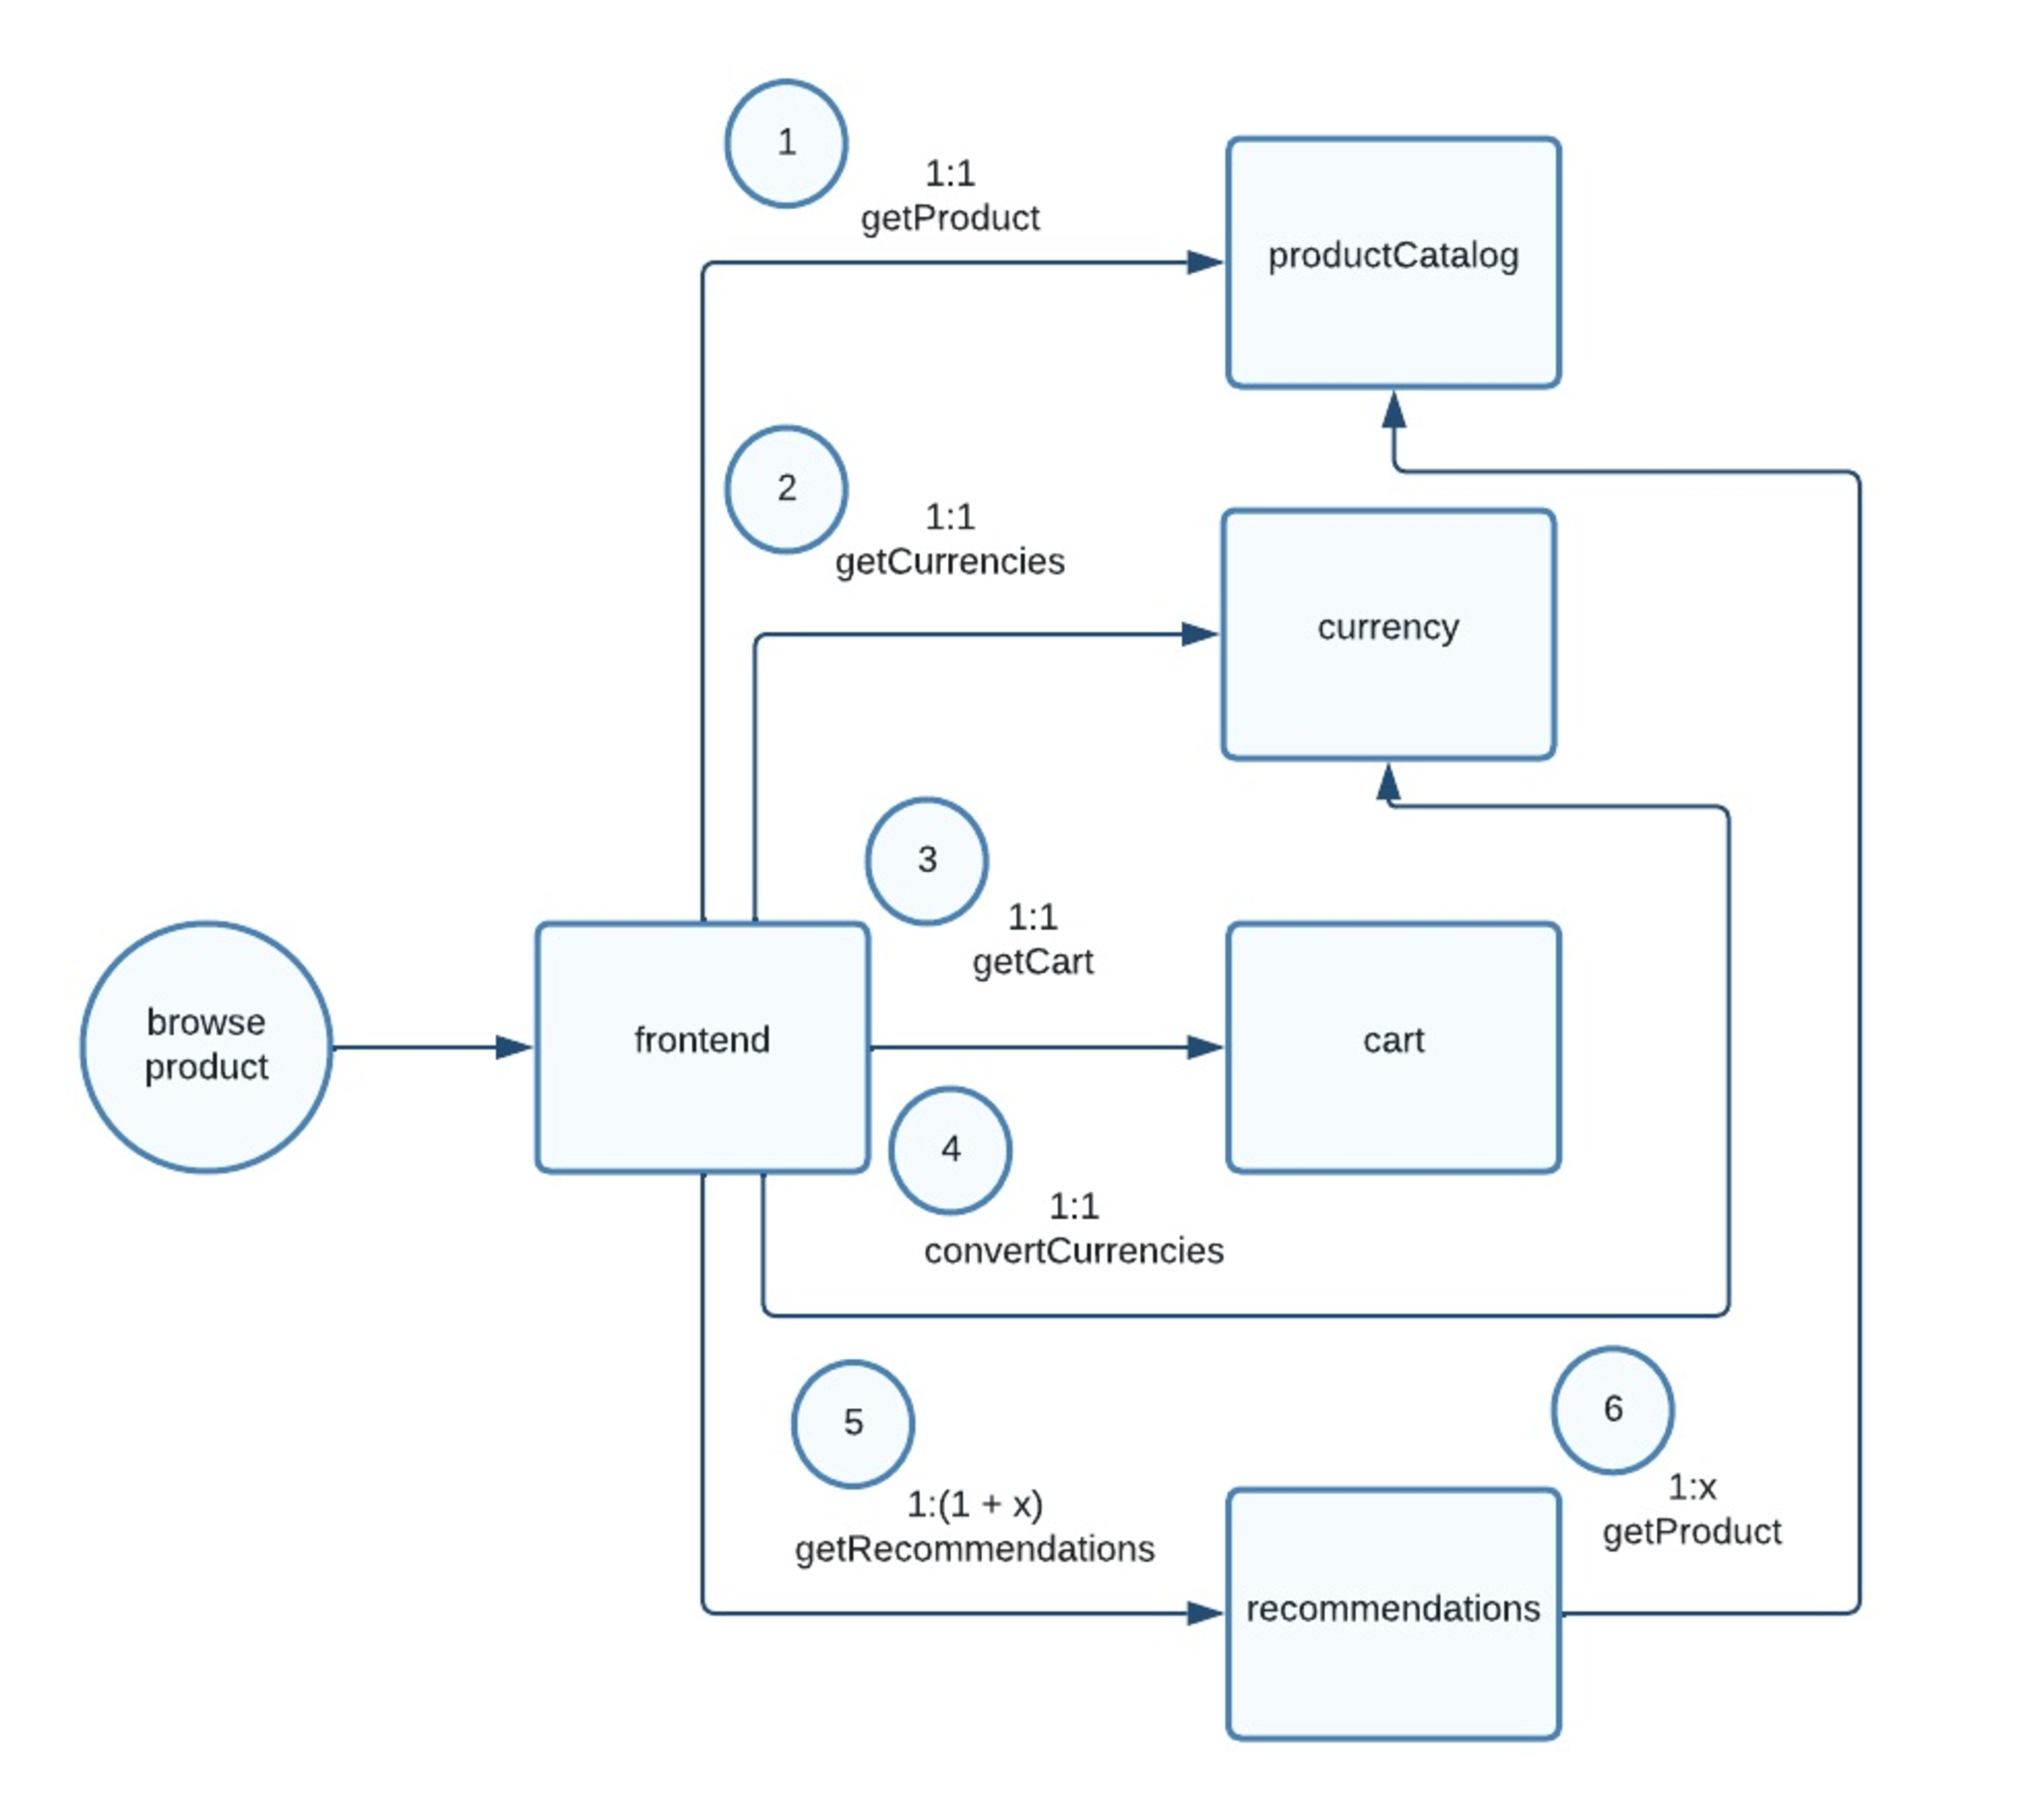
\includegraphics[width=0.5\textwidth]{img/browse-product}
    \caption{browseProduct endpoint: all requests are sequential gRPC 
    with the following order 
    (1) retrieve a list of products from productCatalog service, 
    (2) retrieve latest currrency conversion from currency service, 
    (3) retrieve shopping cart status from cart service, 
    (4) convert currency given the current user setting from currency service,
    (5) retrieve related products from recommendation service,
    (5) retrieve product details for each relate product from productCatalog service.}
    \label{fig:example}
\end{figure}

We use \ours to estimate the throughput improvement of the browseProduct endpoint following optimizing the productCatalog service. 
The profiling results obtained from \ours show that optimizing the productCatalog service by decreasing its processing time for each request by 70\% 
leads to the most effective end-to-end throughput improvement. 
Deploying \ours to profile each individual service or combinations of services offers valuable insights into identifying the most 
impactful targets for optimization, thereby supporting more strategic and effective performance enhancements.
\begin{figure}[h]
    \centering
    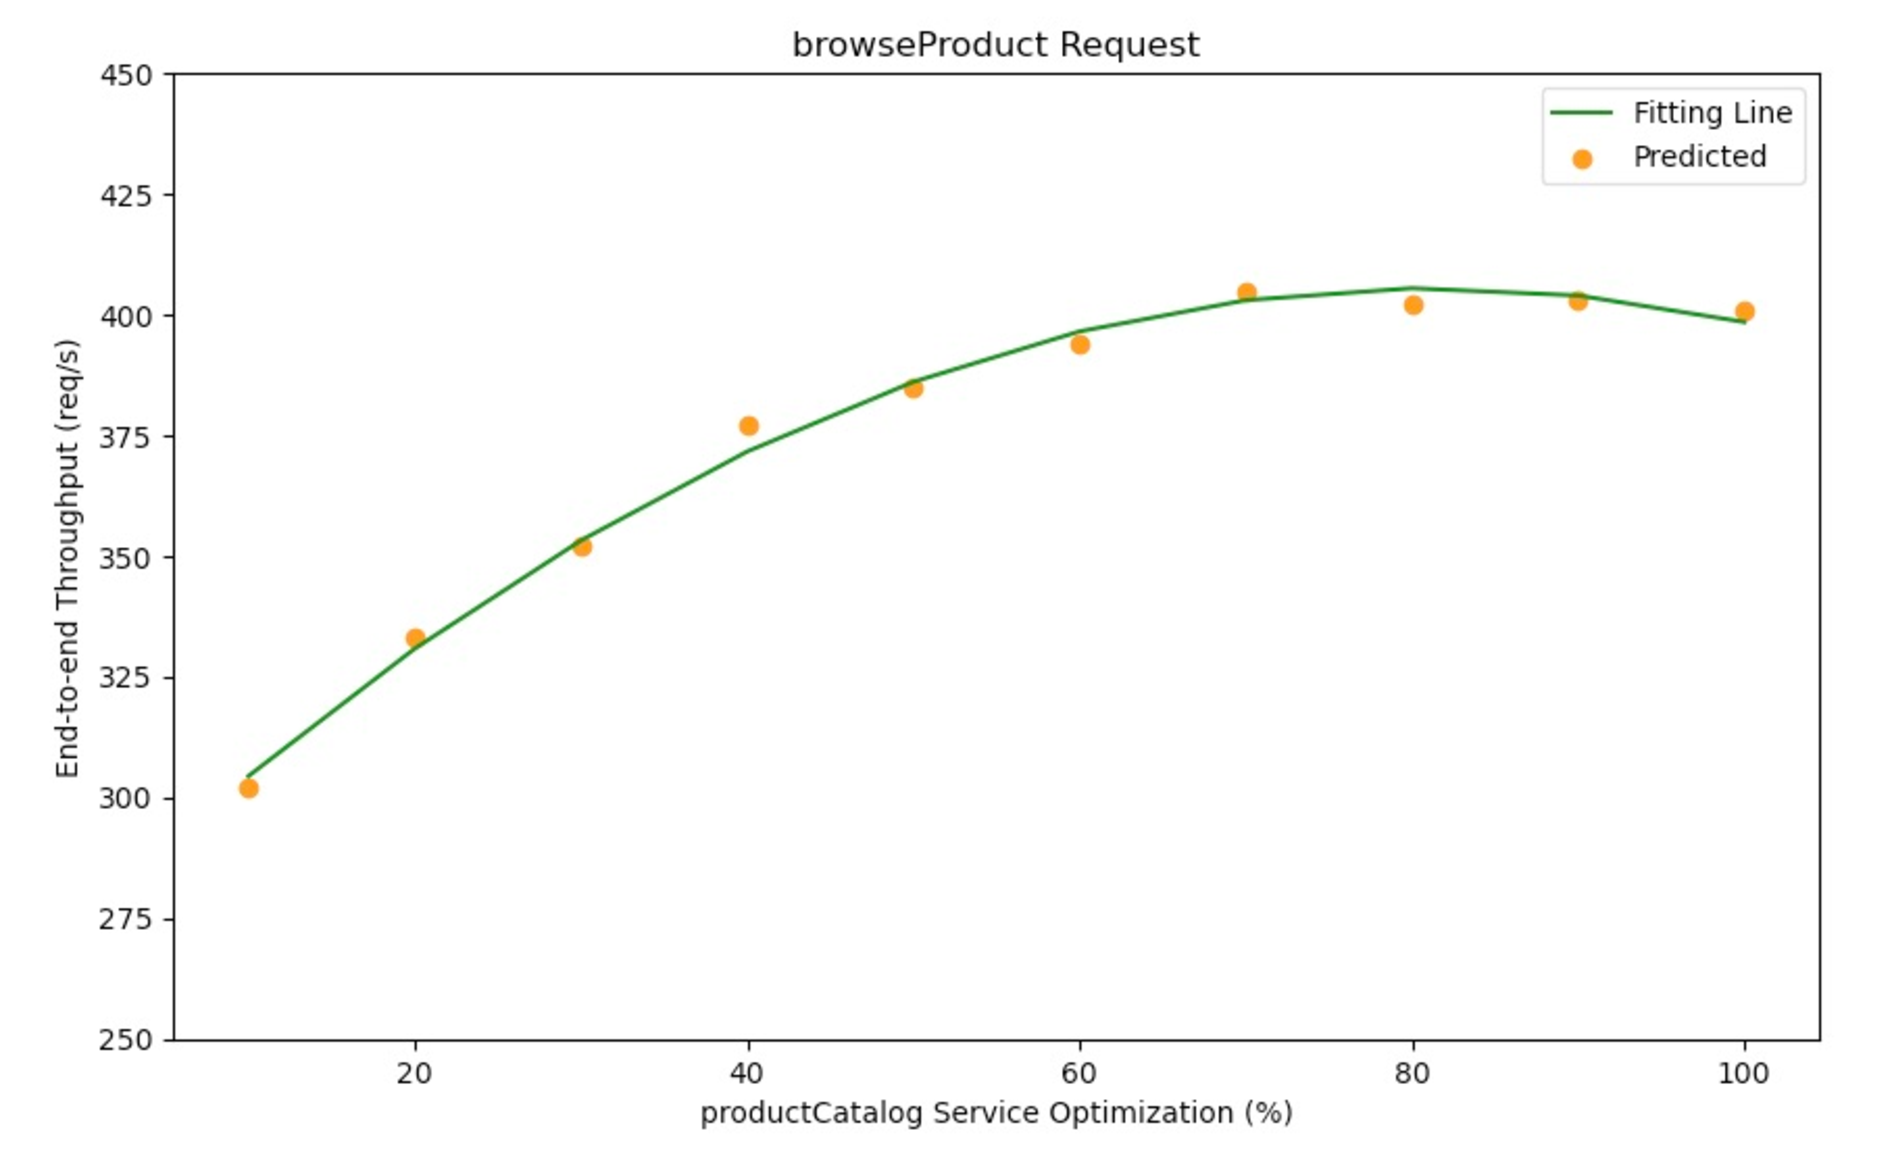
\includegraphics[width=0.5\textwidth]{img/example-output}
    \caption{\ours profiling result for browseProduct request: x axis is the percentage of optimization 
    on productCatalog service, 50\% optimization means the service spend 50\% of the original execution time for each request
    , y axis is the throughput of end-to-end system.}
    \label{fig:example}
\end{figure}

%%%%%%%%%%%%%%%%%%%%%%%%%%%%%%%%%%%%%%%%%%%%%%%%%%%%%%%%%%%%
%%                    System Overview                     %%
%%%%%%%%%%%%%%%%%%%%%%%%%%%%%%%%%%%%%%%%%%%%%%%%%%%%%%%%%%%%

\section{\ours Design}

Slowpoke combines several subsystems: a general and composable performance model incorporating key service interaction 
patterns and their effects, a load-generation and trace-replay subsystem for determining standalone service capacity, 
and a rate-limiting analyzer that calculates the precise effects of an optimization by applying appropriate transformations 
to all distributed components. 

\begin{figure}[h]
    \centering
    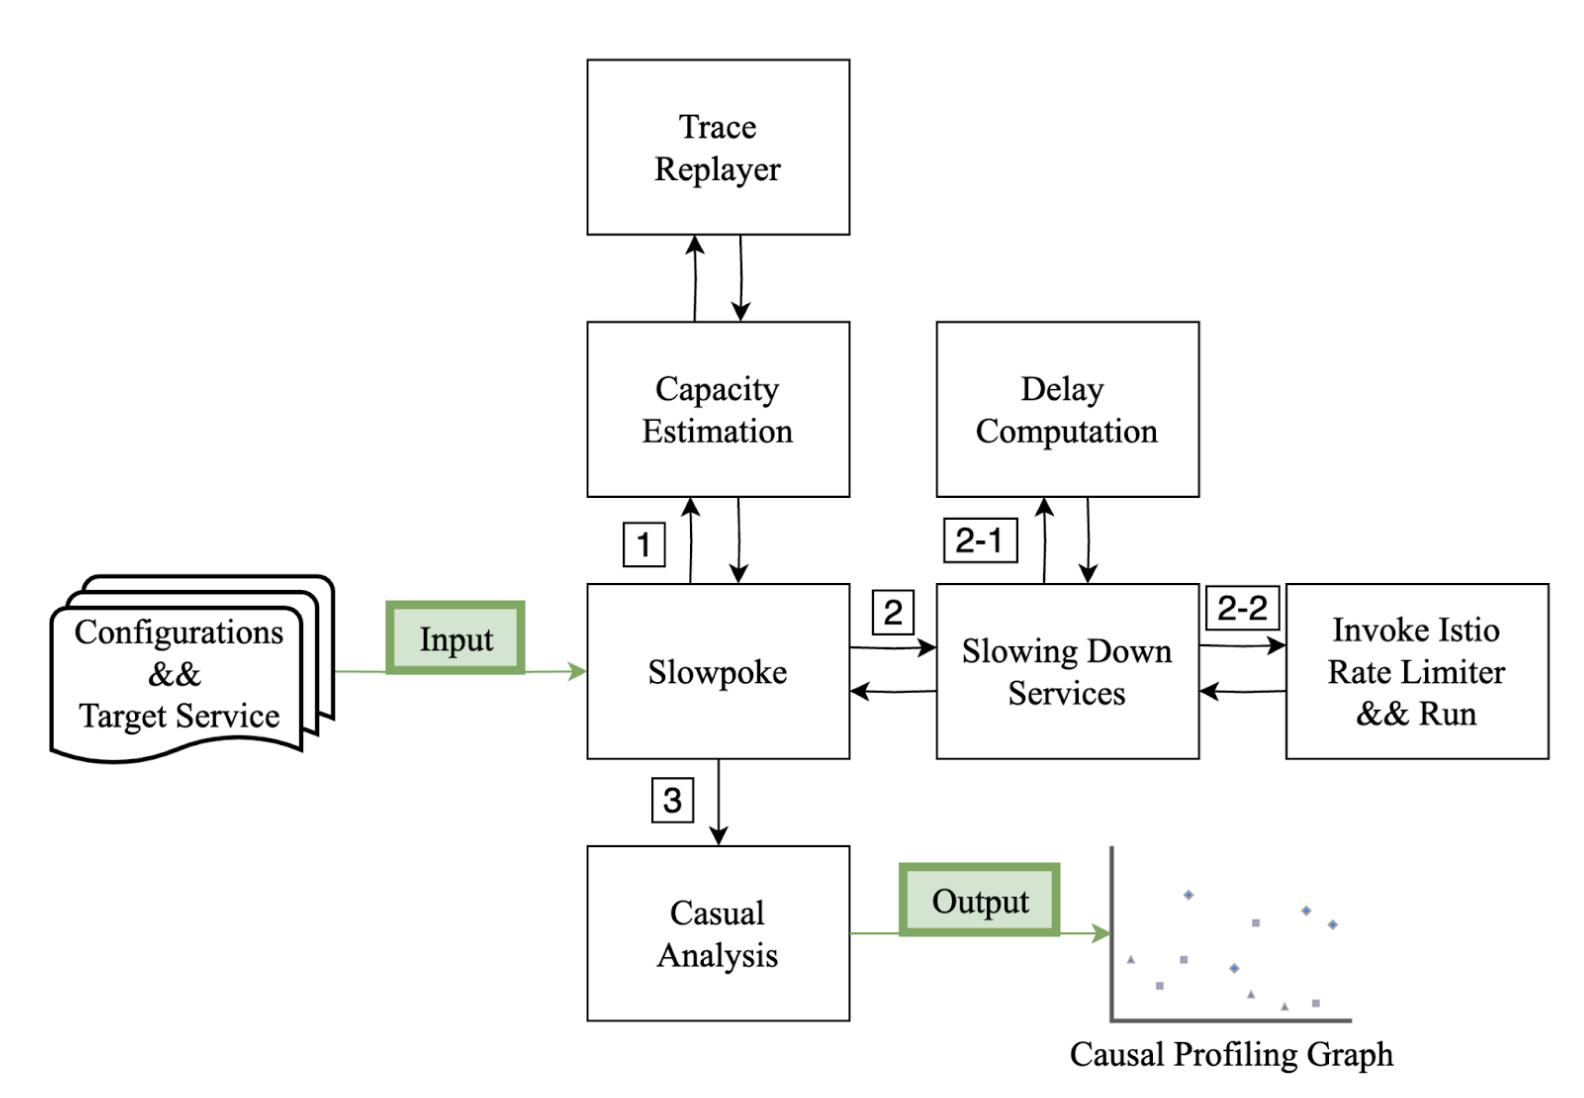
\includegraphics[width=0.5\textwidth]{img/system-overview}
    \caption{\ours Overview }
    \label{fig:example}
\end{figure}

%%%%%%%%%%%%%%%%%%%%%%%%%%%%%%%%%%%%%%%%%%%%%%%%%%%%%%%%%%%%
%%                       Casual Model                     %%
%%%%%%%%%%%%%%%%%%%%%%%%%%%%%%%%%%%%%%%%%%%%%%%%%%%%%%%%%%%%


\begin{figure}[h]
    \centering
    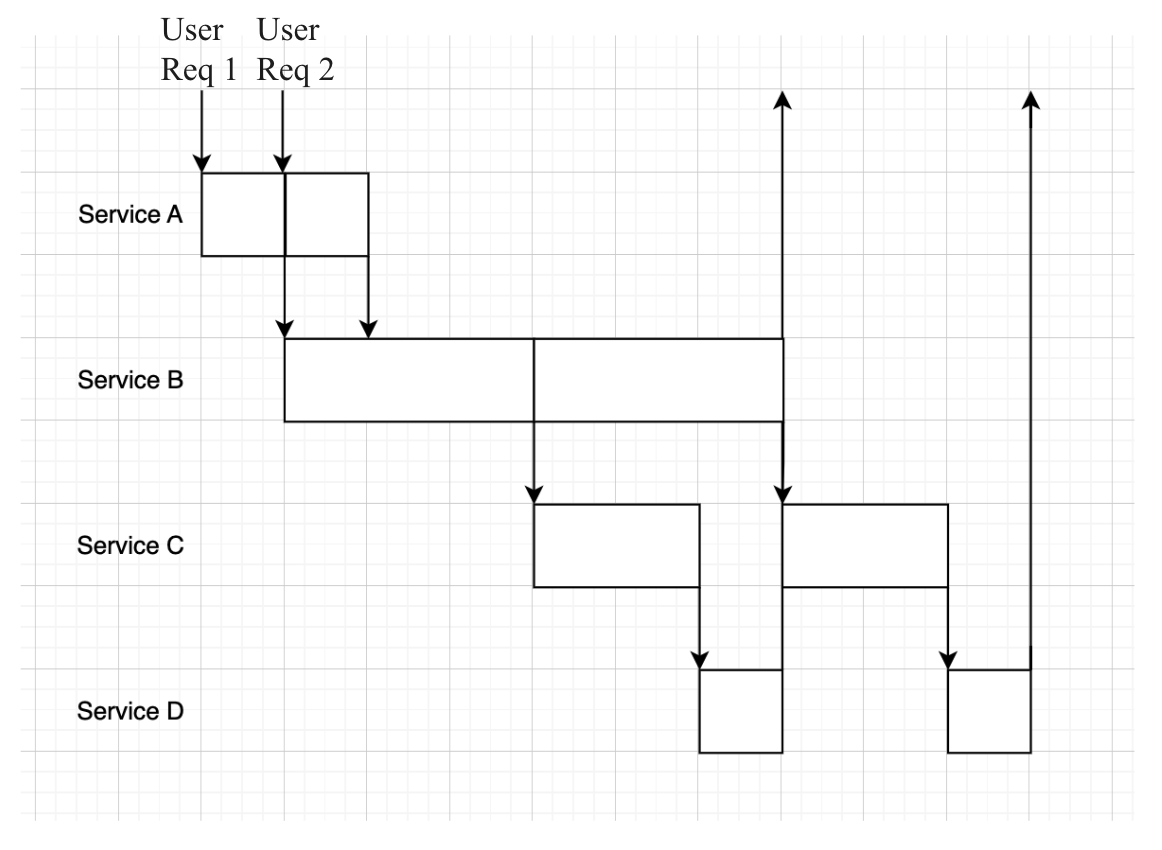
\includegraphics[width=0.5\textwidth]{img/original}
    \caption{Example Execution Graph: each block represents the processing time of the service on each individual user request. Arrow indicates the communication (e.x., HTTP request) between two services.}
    \label{fig:example}
\end{figure}


\stitle{Performance model} 
We use the example depicted in Figure 4 to elucidate the mathematical model. 
In this example, Service A functions as a frontend service, receiving user requests, executing processing tasks for a specified duration, subsequently generating requests to Service B, and waiting replies from Service B before responding to the user.
For simplicity, each service in the example operates is single-threaded. Every user request entails only one internal event across all services.
The throughput of the example application is approximately one request per three time units, as determined by the maximum processing time among all services.
\begin{equation}
    \label{eq:r_origin}
    R_{origin} = \frac{1}{\max(t_A, t_B, t_C, t_D)}
\end{equation}
where $t_S$ is the processing time of each request in service S. Suppose we decrease the processing time of service B (target service) by $\epsilon$ time units. 
Consequently, the throughput of the optimized application improves to approximately one request per two time units:
\begin{equation}
    \label{eq:r_opt}
    R_{opt} = \frac{1}{\max(t_A, t_B-\epsilon, t_C, t_D)}
\end{equation}
where $\epsilon$ is the amount of time units due to optimizing service B.
However, demonstrating such benefits through optimizations requires a considerable investment of time and effort from developers.
The aim of the model is to assess the necessity of investing in the optimization of a particular service.
Instead of optimizing service B directly, we can introduce a delay of $\epsilon$ to slow down all other services except service B. 
The resulting throughput after inserting this delay to all other services is approximately one request per three time units:
\begin{equation}
    \label{eq:r_vs}
    R_{vs} = \frac{1}{\max(t_A+\epsilon, t_B, t_C+\epsilon, t_D+\epsilon)}
\end{equation}
We can connect equation 2 and 3 with the following mathematical transformation:
\begin{gather}
\begin{aligned}
    \frac{1}{R_{opt}} &= \max(t_A, t_B-\epsilon, t_C, t_D) \\
    &= \max(t_A+\epsilon, t_B, t_C+\epsilon, t_D+\epsilon) - \epsilon \\ 
    &= \frac{1}{R_{vs}} - \epsilon
\end{aligned}
\end{gather}
We can predict the throughput after real optimization on target service by using the throughput after slowing down all other services. 
Apply the model on the example, we can infer the throughput after real optimization on service B as one request per two seconds.


% \stitle{Model revision} 
% In above discussion, we insert the same amount of delay as the amount of time units optimized for target service $\epsilon$. 
% However, the delay inserted to each incoming request for service S need to be carefully computed depending on multiple factors:
% the frequency of calls for each service in response to a single user request, dynamic call graphs where some services will be touched depending on the 
% state of the input or system, and the number of enpoints each service exposes. We will further consider these factors in the model to provide 
% more accurate estimation.

\stitle{Capacity estimation} To slow down services, we limit all services except target service with a rate defined by the processing time and delay.
Ideally we can isolate each standalone service and replay the traces fast enough to saturate the service, thereby determining its capacity and 
estimating processing time per request. Now we stick to the quick-n-dirty approach for simplicity: let S be the service 
whose capacity we want to estimate. We allocate one CPU for S and let all other services in the call graph to use as many resources as they need. We increase 
the input rate until service S reaches 100\% CPU utilization and measure observed number of requests per second as the capacity.

\stitle{Istio rate limit}
We use the Istio service mesh \cite{istio} to slow down services through rate limiting.
Istio is a dedicated insfrastructure layer on Kubernetes extending functionalities such as observability and traffic management.
Istio deploys envoy proxy in Kubernetes sidecar container to intercept all network traffic from/to the main application container.
The built-in rate limiter will return an error code for the incoming requests being rate-limited. However, we need to buffer the requests
and release them in a certain rate without requiring users handling reponse with error codes..
To install our logic, we use Istio wasm plugin (C++ SDK) which provides a mechanism to extend the native istio functionalities. 


% \begin{figure}[htbp]
%     \centering
%     \begin{subfigure}[b]{0.35\textwidth}
%         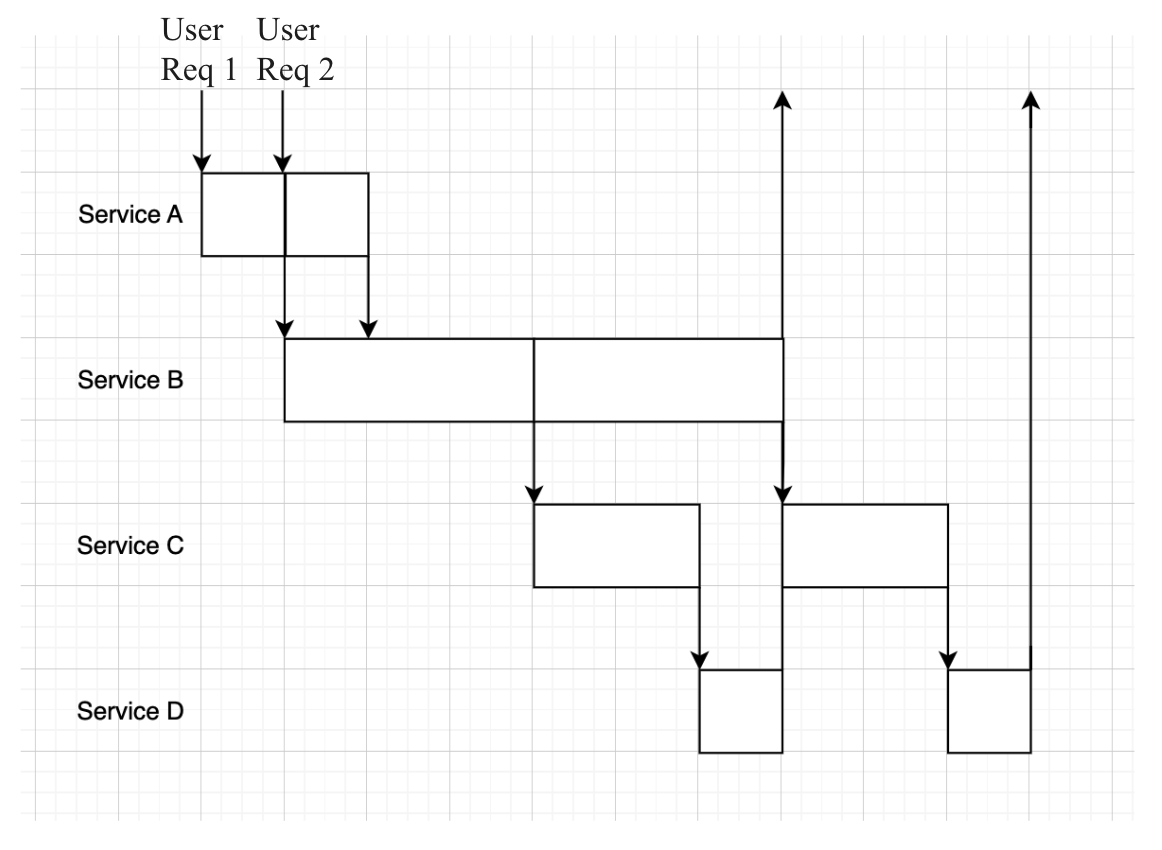
\includegraphics[width=\textwidth]{img/original}
%         \caption{Original execution graph}
%         \label{fig:image1}
%     \end{subfigure}
%     \hfill
%     \begin{subfigure}[b]{0.35\textwidth}
%         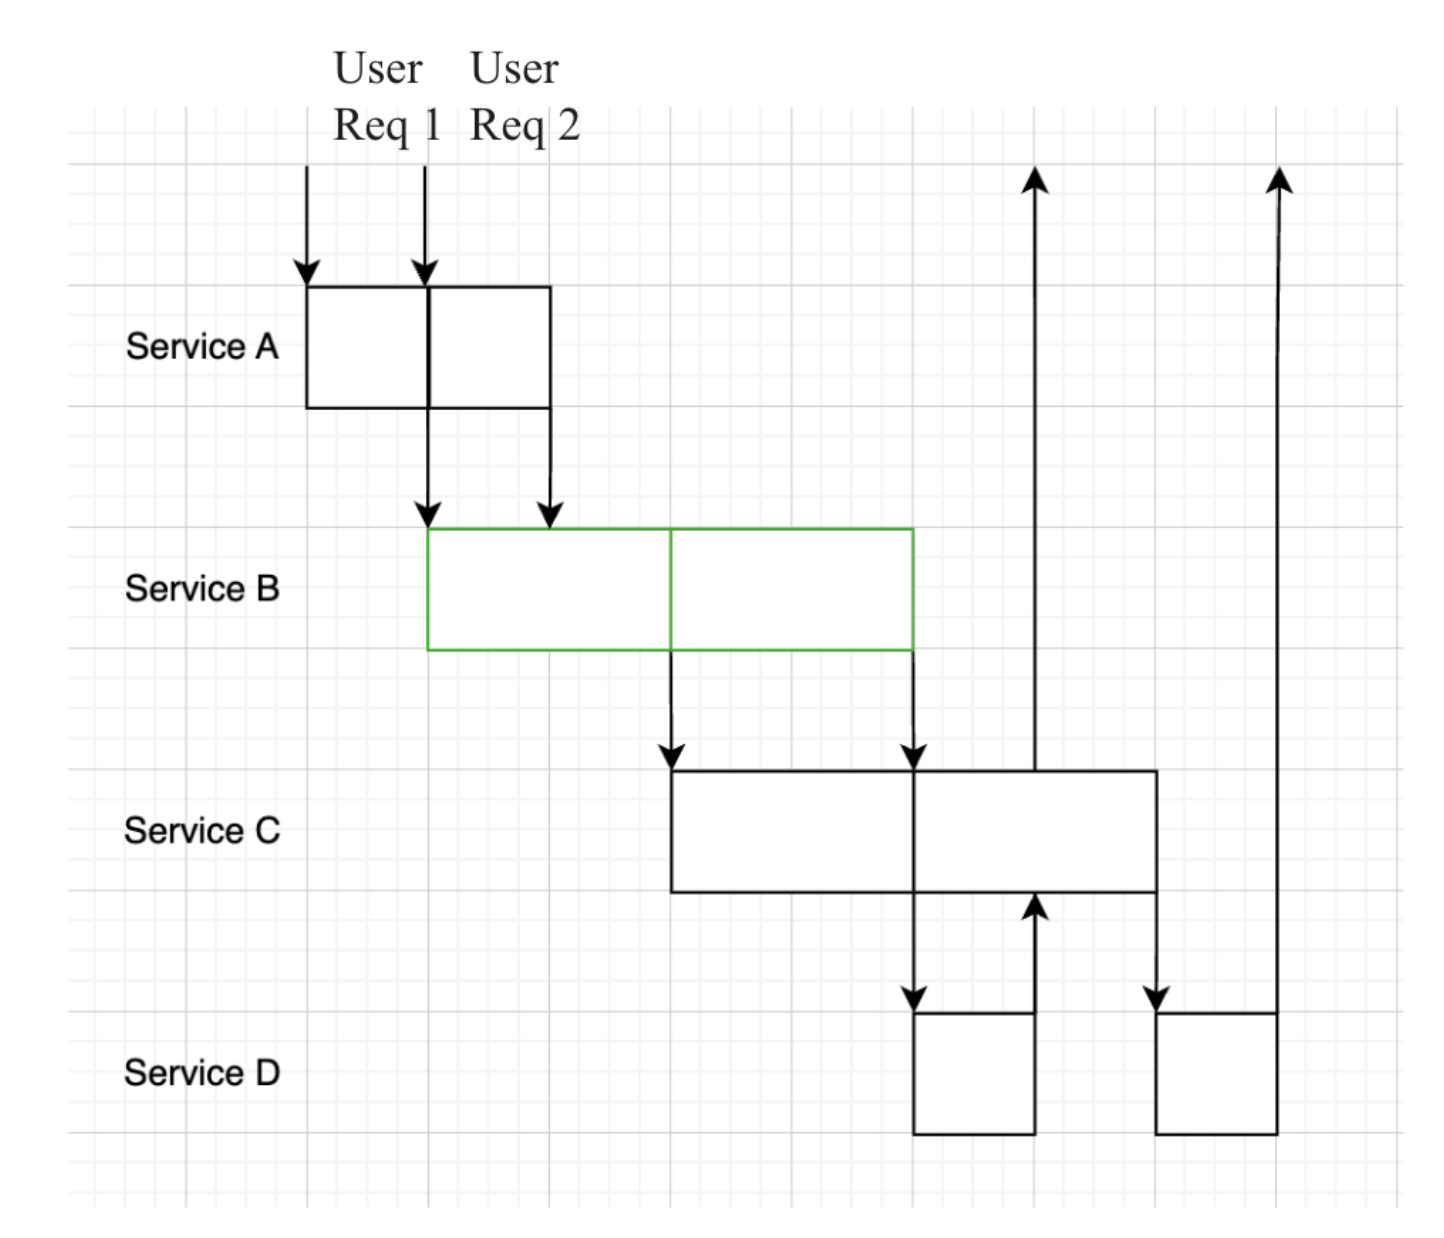
\includegraphics[width=\textwidth]{img/opt}
%         \caption{Optimized execution graph}
%         \label{fig:image2}
%     \end{subfigure}
%     \hfill
%     \begin{subfigure}[b]{0.4\textwidth}
%         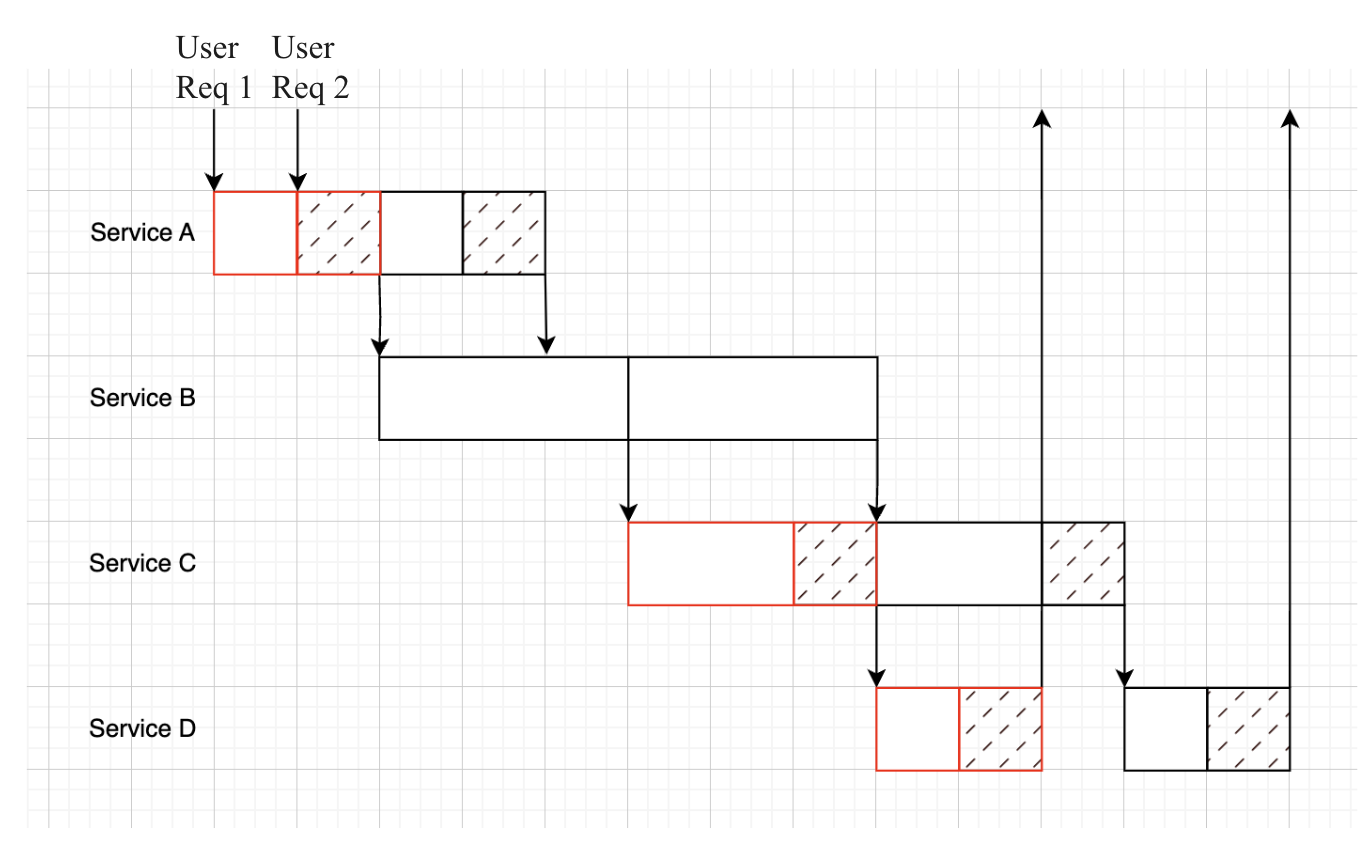
\includegraphics[width=\textwidth]{img/vs}
%         \caption{Delayed execution graph}
%         \label{fig:image3}
%     \end{subfigure}
%     \caption{Execution graphs (a) The original execution graph. In this graph, service A will spend one time units for each incoming request, service B, C, D will spend three, two, one time unit(s) for each incoming request. (b) Assuming we've already optimized service B from three time units to two time units. (c) We insert one time unit for each incoming request for service B, C, D.}
%     \label{fig:three_images}
% \end{figure}


%%%%%%%%%%%%%%%%%%%%%%%%%%%%%%%%%%%%%%%%%%%%%%%%%%%%%%%%%%%%
%%                         Evaluation                     %%
%%%%%%%%%%%%%%%%%%%%%%%%%%%%%%%%%%%%%%%%%%%%%%%%%%%%%%%%%%%%
\section{Evaluation Sketch}
% \paragraph{Benchmarks}
We aim to evaluate \ours on exhaustive exploration of microservice configuration using a combination of real-world and synthetic benchmarks to answer the following questions.
\begin{itemize}
\item Can \ours provide accurate end-to-end throughput improvements estimation across various microservice configurations?
\item How well is \ours estimating the end-to-end throughput improvements with real-world use cases?
\item What are the limitations and overhead of \ours in terms of accuracy and efficiency?
\end{itemize}
We use three real-world benchmarks: \emph{Online-boutique Application} from Google, \emph{Social Network Application} and \emph{Hotel Reservation Application} from DeathStarBench microservices benchmark~\cite{dsb}.
For synthetic benchmarks, we use HydraGen~\cite{hydragen}, a synthetic benchmark generator, to conduct an exhaustive evaluation across a full set of microservice configurations including but not limited to: call graph topology, scale of microservices, 
communication protocol and types of communication (synchronous and asynchronous). 
% \paragraph{Experimental setup} We performed all experiments on CloudLab [XXX] and Chameleon Cloud [XXX] platforms.
% The specific machines used encompass a wide range of configurations using Centos8-Stream with x86 processor architecture between 8-32 vCPUs and 64-256GB of memory.
% Except otherwise noted, all experiments are done using a Kubernetes cluster of $4$ nodes.

% To change resources or images of the services, we delete the namespace and redeploy the benchmark with new configurations.
% We use a combination of wrk (closed-loop) and wrk2 (open-loop) in our experiments, and our capacity estimation methodology varies depending on which workload generator is used.

% \paragraph{Preliminary Results} ?

\section{Proposed Plan}
\stitle{Real-world benchmarks evaluation} 
To achieve rate limiting across all services, we rely on Istio's capabilities for intercepting layer-7 requests. 
However, Istio currently lacks support for certain layer-7 protocols, such as Thrift RPC or Memcached. 
By default, Istio treats these protocols as opaque TCP traffic, hindering our ability to perform request-based rate limiting.
Aeraki \cite{aeraki} is a dedicated project that extends Istio's functionalities to support additional protocols. 
We will implement encoder/decoder support for all required protocols and integrate an equivalent rate limiter within 
Aeraki. 

\stitle{Error analyses} We have observed certain errors in existing results derived from synthetic benchmarks. 
While manipulating cloud infrastructure or workload generators can resolve some of these issues, 
it is essential to investigate the root causes of these errors and develop solutions to mitigate 
them and enhance the accuracy and reliability of \ours.

\stitle{Real optimizations}
To establish the groundtruth following real optimization on the target service, we remove the artificial delays previously added to the services. In real-world 
scenarios, we will execute actual optimizations on the target service and compare the resulting groundtruth against the estimations provided by \ours. Real-world optimizations may involve 
manually optimizing application codes or upgrading the hardware on which the services are running. Notably, \ours should be agnostic to the type of real-world optimization, 
enabling its application across a broad range of performance improvement strategies.


\section{Related Work}
\stitle{Critical path analysis.}
Critical path approaches using end-to-end tracing \cite{mystery_machine, crisp} effectively answer questions such as, \emph{"Where the time is spent?"}.
However, the core challenge is that optimizing a task on the critical path does not guarantee an equivalent improvement in end-to-end performance. 
This is due to the potential emergence of new, previously unseen critical paths following the optimization. 

\stitle{Causal profiling}
Coz \cite{coz} introduced the concept of causal profiling, targeting on multi-threaded single-machine programs. Directly applying Coz's approach to distributed systems, however, presents new challenges. 
For example, coz samples execution threads and insert delays to other execution threads when one thread is executing the optimization section. In a distributed environment, sampling execution and introducing 
delays across all microservices for a specific user request is impractical, as all services are long-running and handle multiple requests concurrently.


\stitle{Microservice Characterization} The characterizations of state-of-the-art large-scale microservice systems by Alibaba \cite{alibaba} and Meta \cite{meta} provide insights of the evaluation of \ours using synthetic benchmarks, offering a deeper understanding of how \ours operates within complex and large-scale microservices architectures.

% \input{introduction}
% \input{overview}
% % \section{Preliminaries}\label{sec:background}

% \subsection{Causal profiling}\label{sec:coz_background}

% \john{Explain virtual speedups and why they make sense.}

% Coz~\cite{coz}, Virtual causal profiling~\cite{virtual_coz}

% \subsection{Service meshes}\label{sec:mesh_background}

% \john{Describe overall service mesh architecture, sidecars, envoy filters, and everything the reader needs to understand the following sections}

% Istio~\cite{istio}, Linkerd~\cite{linkerd}, Cilium~\cite{cilium}, Envoy~\cite{envoy}, \cite{meshes_networking}



% \input{model}
% \input{implementation}
% \input{evaluation}
% \input{related}
% \input{next}
%\input{conclusion}

%%
%% The acknowledgments section is defined using the "acks" environment
%% (and NOT an unnumbered section). This ensures the proper
%% identification of the section in the article metadata, and the
%% consistent spelling of the heading.
%\begin{acks}
%To Robert, for the bagels and explaining CMYK and color spaces.
%\end{acks}

%%
%% The next two lines define the bibliography style to be used, and
%% the bibliography file.
\bibliographystyle{plain}
\bibliography{refs}


%%
%% If your work has an appendix, this is the place to put it.
%\clearpage
%\appendix
%\input{appendix}
%\subsection{Part One}

\end{document}
\endinput
%%
%% End of file `sample-sigconf.tex'.
